\chapter{Law of Flotation}

\section{Aim}
To investigate the relationship between the weight of a floating object and the weight of the water it displaces

\section{Background Information}
It is easier to lift a bucket of water when the bucket is in the water, rather than when it is in air. When an object is floating in water it displaces some water. Therefore there might be a relationship between the weight of the object and the weight of the water it displaces.

\section{Materials}
Eureka can, 1000 mL measuring cylinder, beaker of 100 mL, test tube, beam balance, water, lead shots

\section{Procedure}
\begin{enumerate}
\item Pour water into the large beaker to about $^3/_4$ full.
\item Dip a test tube into the beaker containing water.
\item Put a few small lead shots into the test tube, and add the lead shots slowly until the test tube floats vertically upright in the beaker of water. 
\item Remove the loaded test tube, dry and measure its mass and record this as $m_1$.
\item Pour water into the Eureka can until it just begins to overflow through the spout.
\item Take a small empty dry beaker, measure the mass and record it as $m_2$. Place it under the spout of the Eureka can.
\item Lower the loaded test tube slowly into the Eureka can so that it does not touch the sides.
\item Wait until the displaced water ceases to drop into the weighted beaker.
\item Measure the mass of the beaker with the displaced water and record it as $m_3$.
\end{enumerate}

\begin{figure}[h!]
\centering
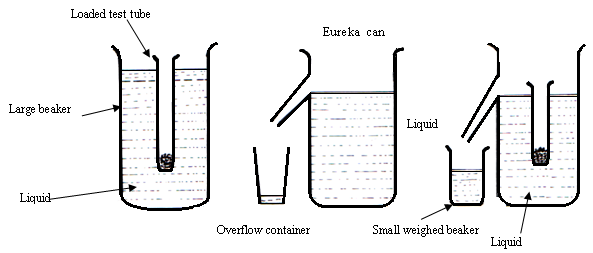
\includegraphics[width=14cm]{./img/law-of-flotation-1.png}
\caption{Law of Flotation practical setup}
\label{fig:law-of-flotation-1}
\end{figure}

\section{Safety Measure}
When adding the lead shots, make sure that the test tube is in a slanted position.

\section{Analysis and Interpretation}
\begin{enumerate}
\item Convert the masses $m_1$, $m_2$, and $m_3$ into weights and call them $w_1$, $w_2$ and $w_3$. 
\item Find the weight of water displaced and record it as $w_4$.
\item What is the relationship between $w_1$ and $w_4$?
\end{enumerate}

\section{Conclusion}
Is there any relationship between the force acting on a floating object and the weight of water displaced by it? Explain.

\section{Questions for Discussion}
\begin{enumerate}
\item Why did the test tube stand upright when the lead shots were added?
\item Why must the loaded test tube float without touching the sides of the beaker?
\item What would happen if the test tube was upright when placed in the water and the lead shots were added?
\end{enumerate}

\section{Reflection and Self Assessment}
\begin{enumerate}
\item What is the importance of the plimsoll line on a ship?
\item How can you use the knowledge you have learned in this experiment in your daily life?
\item Is there anything you did not understand in this experiment? If so, what was it and in what ways can you increase your understanding? 
\end{enumerate}